\documentclass[12pt, a4paper]{article}

% --- PAQUETES ESENCIALES ---
\usepackage[utf8]{inputenc}
\usepackage[T1]{fontenc}
\usepackage[spanish]{babel}
\usepackage{amsmath}
\usepackage{graphicx}
\usepackage{booktabs}
\usepackage{geometry}
\usepackage{hyperref}
\usepackage{fancyhdr}
\usepackage[table]{xcolor}
\usepackage{listings}

% --- ETIQUETA 'LISTING' A 'LISTADO' ---
\addto{\captionsspanish}{\renewcommand{\lstlistingname}{Listado}}
\addto{\captionsspanish}{\renewcommand{\lstlistlistingname}{Listado de Códigos}}

% --- ESTILO DE CÓDIGO ---
\definecolor{GrisClaro}{rgb}{0.95, 0.95, 0.95}

\lstset{
    backgroundcolor=\color{GrisClaro},
    basicstyle=\ttfamily\small,
    breaklines=true,
    showstringspaces=false,
    numbers=left,
    numberstyle=\tiny\color{gray},
    frame=single,
    framesep=5pt,
    rulesepcolor=\color{black},
    keywordstyle=\color{blue}\bfseries,
    commentstyle=\color{green!60!black}\itshape,
    stringstyle=\color{orange},
    tabsize=2,
}

% Definición de lenguajes que listings no trae nativamente
\lstdefinelanguage{Kotlin}{
    keywords={package, import, fun, override, val, var, when, class, return, super, private, public, internal, object, this, if, else, true, false, null, in, is, as},
    keywordstyle=\color{blue}\bfseries,
    ndkeywords={String, Int, Boolean, Unit, Bundle, MethodChannel, FlutterActivity, FlutterEngine, WindowManager},
    ndkeywordstyle=\color{purple}\bfseries,
    sensitive=true,
    comment=[l]{//},
    morecomment=[s]{/*}{*/},
    morestring=[b]",
    morestring=[b]',
}

\lstdefinelanguage{Dart}{
    keywords={import, class, abstract, static, final, const, void, return, if, else, async, await, Future, bool, String, int, double, true, false, null, this, super, extends, new, try, catch, on, in, is, as, override},
    keywordstyle=\color{blue}\bfseries,
    ndkeywords={Widget, State, StatefulWidget, StatelessWidget, BuildContext, MaterialApp, MethodChannel, Platform, PlatformException},
    ndkeywordstyle=\color{purple}\bfseries,
    sensitive=true,
    comment=[l]{//},
    morecomment=[s]{/*}{*/},
    morestring=[b]",
    morestring=[b]',
}

% --- MÁRGENES ---
\geometry{
    a4paper,
    total={170mm,257mm},
    left=25mm,
    right=25mm,
    top=30mm,
    bottom=30mm,
}

% --- ENCABEZADO Y PIE ---
\pagestyle{fancy}
\fancyhf{}
\renewcommand{\headrulewidth}{0pt}
\rfoot{\thepage}
\lfoot{Seguridad de la Información / Miguel Ángel Gutiérrez Gómez}

% --- DATOS DEL DOCUMENTO ---
\newcommand{\nombreuniversidad}{Universidad Politécnica de Chiapas}
\newcommand{\nombrecarrera}{Ingeniería en Software}
\newcommand{\nombremateria}{Seguridad de la Información}
\newcommand{\nombreprofesor}{MC. José Alonso Macías Montoya}
\newcommand{\corte}{Corte 1}
\newcommand{\actividad}{Práctica - Móvil 1 \\ Protección contra Fuga de Información \\ (Prevención de Capturas de Pantalla)}
\newcommand{\nombres}{Miguel Ángel Gutiérrez Gómez}
\newcommand{\matricula}{233382}
\newcommand{\fechaentrega}{\today}
\newcommand{\ciudad}{Suchiapa, Chiapas}

\begin{document}

% --- PORTADA ---
\begin{titlepage}
    \centering
    \vspace*{1cm}
    {\Huge\bfseries \nombreuniversidad \par}
    \vspace{0.5cm}
    {\Large \nombrecarrera \par}

    \vspace{2cm}
    \rule{\textwidth}{1.5pt}
    \vspace{0.4cm}
    {\Large\bfseries \actividad \par}
    \vspace{0.4cm}
    \rule{\textwidth}{1.5pt}

    \vspace{3cm}

    \begin{flushleft}
        \centering
        \textbf{Materia:} \nombremateria \\
        \textbf{Profesor:} \nombreprofesor \\
        \textbf{Corte:} \corte
    \end{flushleft}

    \vspace{0.5cm}

    \begin{flushleft}
        \centering
        \textbf{Alumno:} \nombres \\
        \textbf{Matrícula:} \matricula \\
    \end{flushleft}

    \vfill

    \vspace{1cm}
    \textbf{\ciudad, a \fechaentrega}

\end{titlepage}

\clearpage

% --- ÍNDICE ---
\tableofcontents
\clearpage

% --- CUERPO ---

\section{Introducción}
\label{sec:introduccion}
La fuga de información a través de capturas de pantalla es un vector de ataque
frecuente en aplicaciones móviles que manejan datos sensibles: credenciales,
información financiera, datos personales, expedientes médicos, entre otros.
Una captura puede ser tomada por el propio usuario de forma accidental,
por un atacante con acceso temporal al dispositivo o por software malicioso
que monitorea el contenido en pantalla, y posteriormente compartida sin
control en mensajería, almacenamiento en la nube o vista previa de
multitarea.

El objetivo de esta práctica es construir una vista de inicio de sesión
(\textit{login}) en una aplicación móvil desarrollada con Flutter, mostrar
credenciales de acceso visibles en pantalla, y configurar la ventana de la
aplicación para que sea el propio sistema operativo \textbf{Android} quien
impida activamente la realización de capturas de pantalla mediante la
bandera de seguridad \texttt{FLAG\_SECURE} de \texttt{WindowManager}. El
control debe activarse al entrar a la pantalla protegida y liberarse al
salir, integrándose con el ciclo de vida del widget de Flutter.

\section{Recursos Utilizados}
\label{sec:recursos}
A continuación se listan las herramientas y tecnologías empleadas:

\begin{itemize}
    \item \textbf{SDK:} Flutter 3.44.0 (Dart 3.12.0).
    \item \textbf{Lenguajes:} Dart (capa Flutter) y Kotlin (capa nativa Android).
    \item \textbf{Plataforma objetivo:} Android (API \texttt{WindowManager}).
    \item \textbf{API de seguridad:} \texttt{WindowManager.LayoutParams.FLAG\_SECURE} del sistema operativo Android.
    \item \textbf{Mecanismo de interoperación:} \texttt{MethodChannel} de Flutter para invocar código nativo Kotlin.
    \item \textbf{Editor:} Visual Studio Code con extensiones de Flutter y Dart.
    \item \textbf{Entorno de pruebas:} Emulador Android Studio y dispositivo físico Android.
    \item \textbf{Control de versiones:} Git.
\end{itemize}

\section{Desarrollo}
\label{sec:desarrollo}

\subsection{Justificación de la bandera \texttt{FLAG\_SECURE}}
Android expone, dentro de \texttt{android.view.WindowManager.LayoutParams},
la bandera \texttt{FLAG\_SECURE}. Cuando se aplica a la ventana de una
\texttt{Activity}, el sistema operativo aplica las siguientes restricciones
de forma activa, sin intervención de la aplicación:

\begin{itemize}
    \item Bloquea capturas de pantalla manuales (combinación de
    \textit{volumen abajo} + \textit{encendido}), mostrando un mensaje del
    tipo \textit{``No se puede tomar la captura debido a la política de
    seguridad''}.
    \item Oculta el contenido en la vista de aplicaciones recientes
    (\textit{multitarea}), reemplazándolo por una vista en negro.
    \item Bloquea la grabación de pantalla del sistema.
    \item Impide la proyección de la ventana a pantallas no seguras
    (Cast, salida HDMI no protegida, etc.).
\end{itemize}

A diferencia de soluciones a nivel aplicación que solo \textit{detectan}
una captura ya ocurrida, \texttt{FLAG\_SECURE} la \textbf{previene} en el
compositor de ventanas del propio sistema operativo, por lo que cumple
con el requisito de la práctica: que sea el SO quien impida activamente
la captura.

\subsection{Por qué se requiere código nativo}
El framework de Flutter no expone \texttt{FLAG\_SECURE} a través de su API
pública en Dart, dado que es una funcionalidad específica de la ventana
nativa de Android (no existe equivalente directo en iOS). Para aplicarla
sin depender de paquetes externos se utilizó un \texttt{MethodChannel},
mecanismo oficial de Flutter para invocar código de la plataforma anfitriona
desde Dart.

\subsection{Arquitectura de la solución}
La solución se compone de tres piezas que cooperan:

\begin{enumerate}
    \item \textbf{Capa nativa Android} (\texttt{MainActivity.kt}):
    aplica \texttt{FLAG\_SECURE} en \texttt{onCreate} y registra un
    \texttt{MethodChannel} con los métodos \texttt{enable} y \texttt{disable}.
    \item \textbf{Servicio Dart} (\texttt{secure\_screen.dart}):
    envuelve el canal con dos funciones estáticas que invocan los
    métodos nativos. En plataformas distintas a Android la operación es
    silenciosa (\textit{no-op}).
    \item \textbf{Integración con ciclo de vida del widget}
    (\texttt{login\_screen.dart}): activa la protección en
    \texttt{initState}, la libera en \texttt{dispose} y vuelve a liberarla
    al navegar fuera del login tras un inicio de sesión exitoso.
\end{enumerate}

\subsection{Aplicación de la bandera en el ciclo de vida}
La pantalla de login es un \texttt{StatefulWidget}. El ciclo de vida
aprovechado es:

\begin{itemize}
    \item \texttt{MainActivity.onCreate}: activa \texttt{FLAG\_SECURE}
    inmediatamente al crearse la ventana, de modo que el primer fotograma
    visible ya esté protegido (red de seguridad ante cualquier latencia
    del canal asíncrono).
    \item \texttt{LoginScreen.initState}: llama a \texttt{SecureScreen.enable()};
    re-aplica la bandera si el usuario navegó de vuelta al login tras un
    cierre de sesión.
    \item \texttt{LoginScreen.dispose}: llama a \texttt{SecureScreen.disable()}
    para liberar la restricción al destruirse la pantalla, permitiendo
    que otras pantallas (no sensibles) sí puedan capturarse si así se
    desea.
    \item Submit exitoso: invoca \texttt{disable()} antes de
    \texttt{pushReplacement} a la pantalla principal.
\end{itemize}

\subsection{Implementación}

A continuación se muestran los fragmentos de código clave que materializan
la solución descrita.

\begin{lstlisting}[language=Kotlin, caption={Capa nativa: aplicación de FLAG\_SECURE y registro del MethodChannel}, label={lst:mainactivity}]
package com.example.scanbuild

import android.os.Bundle
import android.view.WindowManager
import io.flutter.embedding.android.FlutterActivity
import io.flutter.embedding.engine.FlutterEngine
import io.flutter.plugin.common.MethodChannel

class MainActivity : FlutterActivity() {
    private val channelName = "visionprice/secure_screen"

    override fun configureFlutterEngine(flutterEngine: FlutterEngine) {
        super.configureFlutterEngine(flutterEngine)
        MethodChannel(flutterEngine.dartExecutor.binaryMessenger, channelName)
            .setMethodCallHandler { call, result ->
                when (call.method) {
                    "enable" -> {
                        runOnUiThread {
                            window.setFlags(
                                WindowManager.LayoutParams.FLAG_SECURE,
                                WindowManager.LayoutParams.FLAG_SECURE
                            )
                            result.success(true)
                        }
                    }
                    "disable" -> {
                        runOnUiThread {
                            window.clearFlags(WindowManager.LayoutParams.FLAG_SECURE)
                            result.success(true)
                        }
                    }
                    else -> result.notImplemented()
                }
            }
    }

    override fun onCreate(savedInstanceState: Bundle?) {
        super.onCreate(savedInstanceState)
        window.setFlags(
            WindowManager.LayoutParams.FLAG_SECURE,
            WindowManager.LayoutParams.FLAG_SECURE
        )
    }
}
\end{lstlisting}

\begin{lstlisting}[language=Dart, caption={Servicio Dart que envuelve el MethodChannel}, label={lst:secure}]
import 'dart:io';
import 'package:flutter/services.dart';

class SecureScreen {
  static const _channel = MethodChannel('visionprice/secure_screen');

  static Future<void> enable() async {
    if (!Platform.isAndroid) return;
    try {
      await _channel.invokeMethod('enable');
    } on PlatformException {
      // Canal no disponible en este build - silencioso
    }
  }

  static Future<void> disable() async {
    if (!Platform.isAndroid) return;
    try {
      await _channel.invokeMethod('disable');
    } on PlatformException {
      // Canal no disponible en este build - silencioso
    }
  }
}
\end{lstlisting}

\begin{lstlisting}[language=Dart, caption={Integración con el ciclo de vida de la pantalla de login (fragmento relevante)}, label={lst:lifecycle}]
class _LoginScreenState extends State<LoginScreen> {
  final _formKey = GlobalKey<FormState>();
  final _emailCtrl = TextEditingController(text: 'miguel.angel@obra.mx');
  final _passwordCtrl = TextEditingController(text: 'password123');

  @override
  void initState() {
    super.initState();
    SecureScreen.enable();
  }

  @override
  void dispose() {
    SecureScreen.disable();
    _emailCtrl.dispose();
    _passwordCtrl.dispose();
    super.dispose();
  }

  void _submit() {
    if (!_formKey.currentState!.validate()) return;
    SecureScreen.disable();
    Navigator.of(context).pushReplacementNamed('/home');
  }
}
\end{lstlisting}

\subsection{Evidencia visual}
La Figura \ref{fig:login} muestra la pantalla de login con las credenciales
visibles que se busca proteger. La Figura \ref{fig:bloqueo} muestra el
resultado al intentar realizar una captura de pantalla en el emulador con
\texttt{FLAG\_SECURE} activo.

\begin{figure}[h]
    \centering
    % 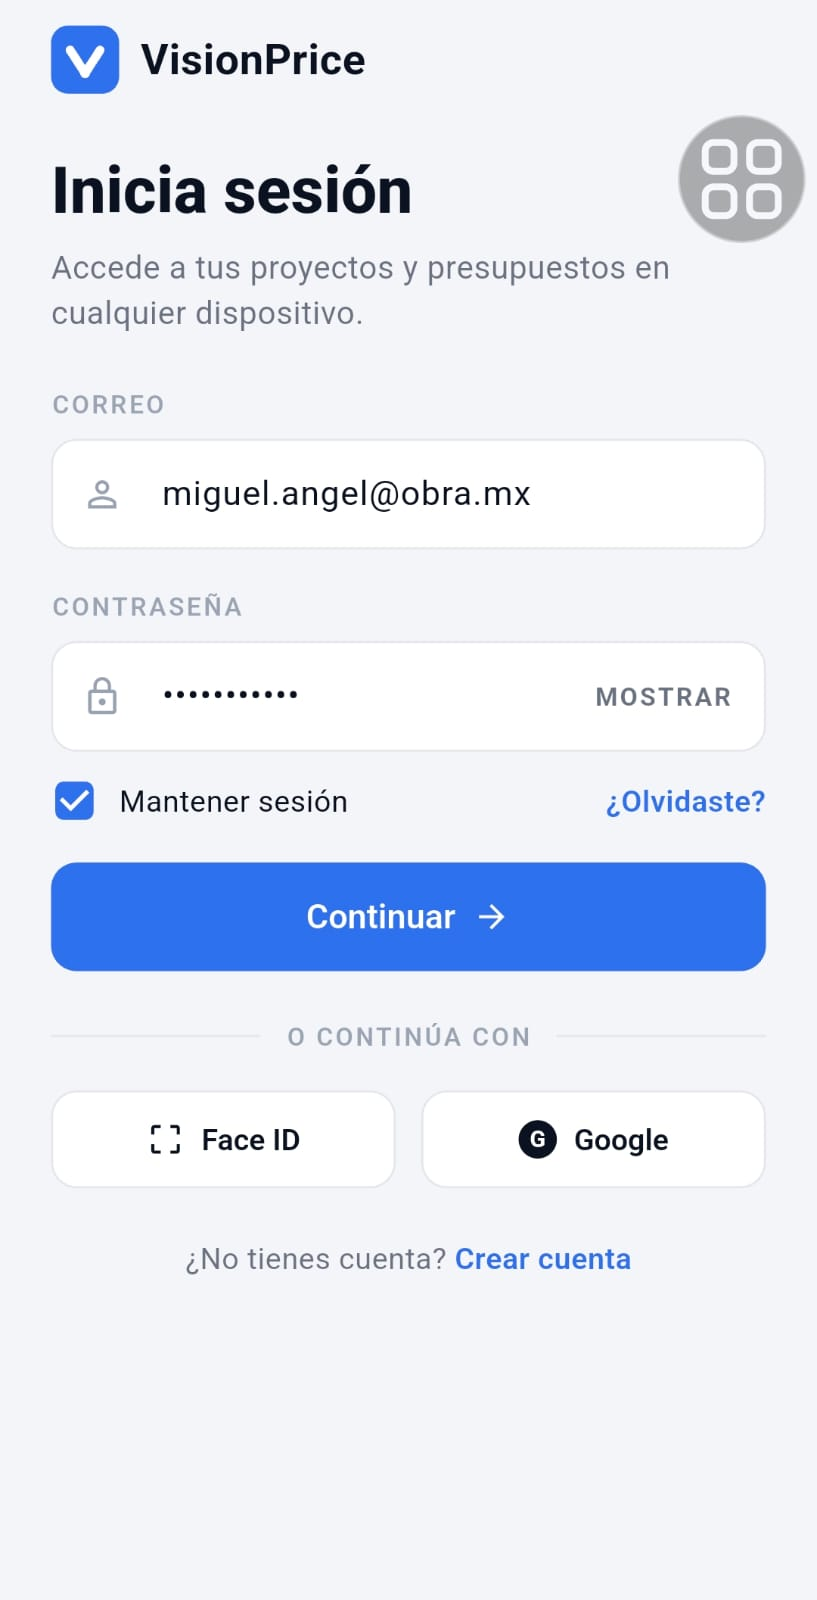
\includegraphics[width=0.45\textwidth]{login.png}
    \fbox{\parbox[c][6cm][c]{0.45\textwidth}{\centering \textit{Captura del login con credenciales visibles}}}
    \caption{Pantalla de inicio de sesión de VisionPrice con credenciales prellenadas.}
    \label{fig:login}
\end{figure}

\begin{figure}[h]
    \centering
    % \includegraphics[width=0.45\textwidth]{bloqueo.png}
    \fbox{\parbox[c][6cm][c]{0.45\textwidth}{\centering \textit{Captura mostrando el toast del SO o la imagen en negro}}}
    \caption{Bloqueo activo del sistema operativo al intentar capturar la pantalla protegida.}
    \label{fig:bloqueo}
\end{figure}

\section{Resultados y Conclusiones}
\label{sec:resultados}

\subsection{Resultados}
Tras compilar la aplicación e instalarla en un dispositivo Android se
verificaron los siguientes comportamientos en la pantalla de login:

\begin{itemize}
    \item \textbf{Captura manual bloqueada:} al ejecutar la combinación
    de volumen abajo + encendido, el sistema operativo despliega el aviso
    \textit{``No se pudo capturar la pantalla''} y no se genera ningún
    archivo de imagen.
    \item \textbf{Multitarea protegida:} al abrir la vista de aplicaciones
    recientes, la vista previa de la app aparece en negro en lugar de
    mostrar el contenido del login.
    \item \textbf{Grabación de pantalla impedida:} la grabación de pantalla
    del sistema produce un video en negro durante el tiempo que la
    pantalla protegida está visible.
    \item \textbf{Liberación al navegar:} tras un \texttt{submit} exitoso,
    la siguiente pantalla (\texttt{HomeShell}) sí permite capturas, lo
    que confirma que el toggle del ciclo de vida funciona como se
    diseñó.
\end{itemize}

\subsection{Conclusiones}
\begin{itemize}
    \item Se cumplió el objetivo de la práctica: construir una vista de
    login con credenciales visibles y garantizar que sea el sistema
    operativo Android quien impida las capturas mediante
    \texttt{FLAG\_SECURE}.
    \item La integración con el ciclo de vida del widget
    (\texttt{initState}/\texttt{dispose}) permite limitar la protección
    a las pantallas que realmente la requieren, evitando degradar la
    experiencia en pantallas no sensibles.
    \item La elección de un \texttt{MethodChannel} directo sobre un
    paquete externo reduce dependencias y mantiene el control sobre el
    código de seguridad.
    \item Es importante reconocer la limitación de iOS: Apple no expone
    una API equivalente que prevenga la captura; únicamente permite
    detectarla mediante notificaciones del sistema. Para protección
    multiplataforma equivalente sería necesario complementar con un
    \textit{overlay} oscuro disparado por dicha notificación.
\end{itemize}

\clearpage

\section{Anexos}
\label{sec:anexos}

\subsection{Repositorio del proyecto}
El proyecto Flutter completo (incluyendo la pantalla de login, el servicio
\texttt{SecureScreen} y la configuración nativa Android) se encuentra en el
directorio \texttt{scanbuild/} adjunto a esta entrega.

\subsection{Estructura de archivos relevantes}

\begin{lstlisting}[language={}, caption={Archivos clave de la solución de seguridad}]
scanbuild/
  android/app/src/main/kotlin/com/example/scanbuild/
    MainActivity.kt              <-- Aplica FLAG_SECURE y expone MethodChannel
  lib/
    main.dart                    <-- Rutas de la app
    services/
      secure_screen.dart         <-- Wrapper Dart del MethodChannel
    screens/
      login_screen.dart          <-- Pantalla protegida (initState / dispose)
\end{lstlisting}

\subsection{Evidencia adicional de bloqueo}
A continuación se reserva espacio para capturas complementarias del emulador
y/o dispositivo físico mostrando el bloqueo en distintos escenarios
(captura manual, multitarea en negro, grabación de pantalla).

\begin{figure}[h]
    \centering
    % \includegraphics[width=0.45\textwidth]{multitarea_negra.png}
    \fbox{\parbox[c][6cm][c]{0.45\textwidth}{\centering \textit{Vista de multitarea con la app en negro}}}
    \caption{Vista de aplicaciones recientes mostrando la app protegida en negro.}
    \label{fig:multitarea}
\end{figure}

\end{document}
